
%----------------------------------------------------------------------------------------
%	inductive coupling
%----------------------------------------------------------------------------------------
\newcommand*{\inductiveCoupling}{\begingroup
\section{Induktive Kopplung}\label{sec:inductivecloupling}
{\noindent Die induktive Kopplung ist eine Art der kontaktlosen Energieübertragung welche sich hauptsächlich in der Anwendung in der Übertragung mit Langwellen und Kurzwellen wiederfindet\footnote{Finkenzeller: RFID Handbuch, S. 69}. Eine induktive Kopplung zweier Spulen liegt dann vor, wenn das sich ändernde Magnetfeld der einen Spule in der anderen Spule eine Spannung induziert\footnote{Stiny, Leonard: Grundwissen Elektrotechnik. 5. Auflage: Franzis Verlag GmbH, S. 100}. Abhängig ist dieses Magnetfeld vom Stromfluss im Leiter und wird als magnetische Feldstärke \textbf{H} bezeichnet.

\magneticFieldStrength
\magneticFluxDensity
\antennaDesign
}
\endgroup}
%----------------------------------------------------------------------------------------


%----------------------------------------------------------------------------------------
%	magnetic field stength
%----------------------------------------------------------------------------------------
\newcommand*{\magneticFieldStrength}{\begingroup
\subsection{Magnetische Feldstärke}\label{sec:magneticfieldstrength}
{\noindent Die magnetische Feldstärke \textbf{H} an einem bestimmten Punkt \textbf{p} ausgehend von einem Leiter \textbf{L} lässt sich für verschiedene Leiterformen rechnerisch ermitteln. In allgemeiner Form gilt, das Umlaufintegral der magnetischen Feldstärke \textbf{H} längs einer geschlossenen Kurve ist gleich der Summe der Stromstärken der eingeschlossenen Ströme\footnote{Finkenzeller: RFID Handbuch, S. 70}.

\begin{equation}
  \sum I = \oint\vec{H} \cdot d\vec{l}
\end{equation}



\clearpage

\begin{wrapfigure}{r}{0.5\textwidth}
    \begin{minipage}[r]{0.5\textwidth}
      \vspace{-16pt}
      \begin{figure}[H]
        \centering
        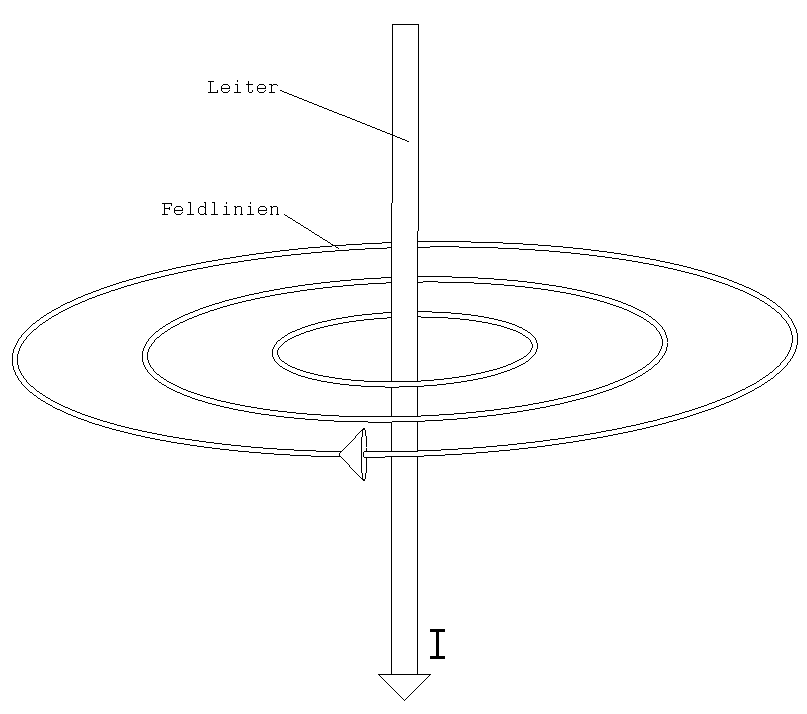
\includegraphics[width=\textwidth]{Graphics/geraderLeiter.png}
        \caption{Feldlinien eines geraden Leiters}{}
        \label{fieldStrengthStraight}
      \end{figure}
      \begin{figure}[H]
        \centering
        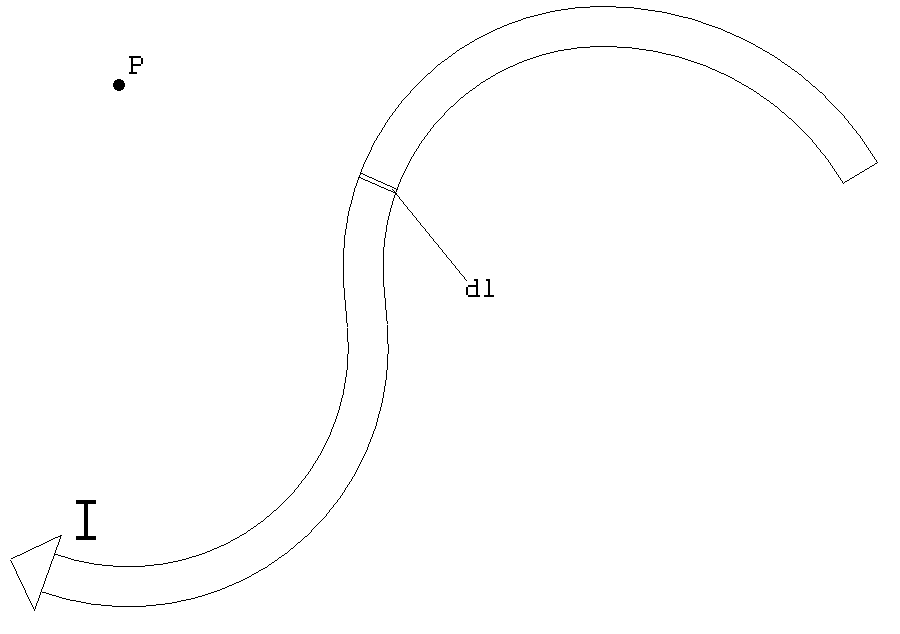
\includegraphics[width=\textwidth]{Graphics/Leiter.png}
        \caption{gebogener Leiter}{}
        \label{fieldStrengthCurved}
      \end{figure}    
      \begin{figure}[H]
        \centering
        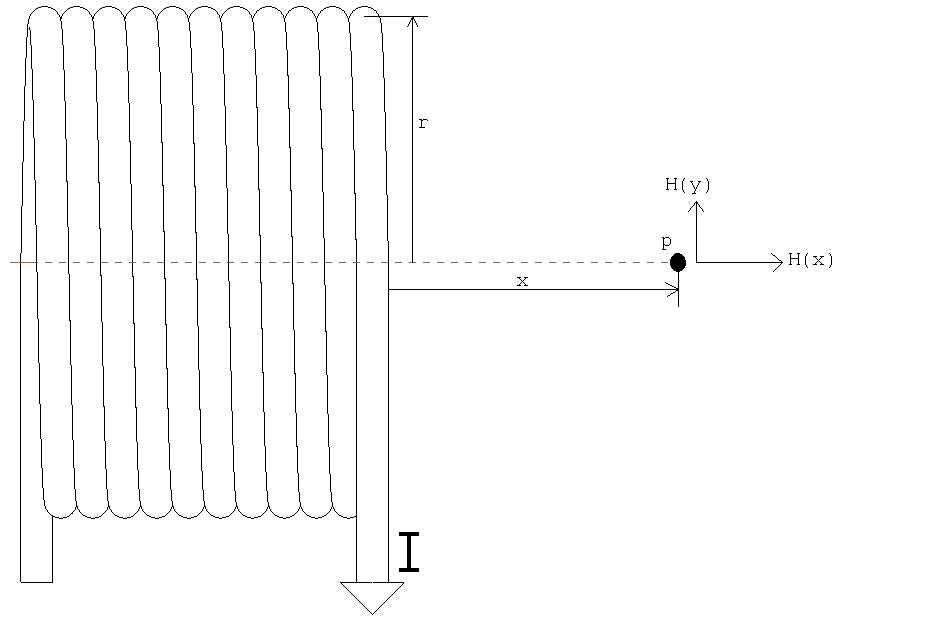
\includegraphics[width=1.2\textwidth]{Graphics/Spule.png}
        \caption{Spule}{}
        \label{coil}
      \end{figure}
    \vspace{-10pt}    
    \end{minipage}  
\end{wrapfigure}
\noindent Für einen geraden Zylindrischen Leiter (Abbildung \ref{fieldStrengthStraight}) gilt, dass die Feldstärke entlang einer kreisförmigen Feldlinie im Abstand \textbf{r} konstant ist und

\begin{equation}
  \oint d\vec{s} = 2\pi \cdot r
\end{equation}

\noindent aufgrund der Zylindrizität. Wird der Leiter also von einem konstanten Strom \textbf{I} durchflossen, so gilt

\begin{equation}
  H = \frac{I}{2\pi \cdot r}
\end{equation}

\noindent Auf Höhe des Leiters ist die Feldstärke \textbf{H} somit ausschließlich vom Abstand \textbf{r} abhängig. Schwieriger ist die Betrachtung eines zylindrischen Leiters wenn dieser nicht einer Geraden entspricht. Die Feldstärke \(d\vec{H}\) an einem Punkt \textbf{p}, ausgehend von einem Leiterstück \textbf{dl}, wie in Abbildung \ref{fieldStrengthCurved} dargestellt, lässt sich mithilfe des Gesetz von Biot und Savart ermitteln

\begin{equation}
  d\vec{H} = \frac{I}{4\pi} \cdot \frac{d\vec{l} \times \vec{p}}{p^3}
\end{equation}

\noindent Die resultierende Feldstärke \(\vec{H}_p\), ausgehend vom gesamten Leiter \textbf{L}, errechnet sich durch integrieren dieser Teilergebnisse 

\begin{equation}
  \vec{H}_p = \frac{I}{4\pi} \cdot \int\limits_L \frac{d\vec{l} \times \vec{p}}{p^3}
\end{equation}

\noindent Nimmt der Leiter \textbf{L} die Form einer Spule mit N Windungen an, so gilt

\begin{equation}
  \vec{H}_p = \frac{N \cdot I}{4\pi} \cdot \oint\limits_L \frac{d\vec{l} \times \vec{p}}{p^3}
  \label{eq:savatCoil}
\end{equation}

\noindent im Folgenden soll die Feldstärke \textbf{H} ausgehend von der Spule ausschließlich auf der Mittelachse der Spule mit einem Abstand \(x > 0\) betrachtet werden (Abbildung \ref{coil}), sodass gilt

\begin{equation}
  p = \left(\begin{array}{c} x \\ 0 \\ 0 \end{array}\right)
\end{equation}

\clearpage

\noindent Unter dieser Bedingung sind die folgenden drei Eigenschaften erfüllt: 

\begin{enumerate}
  \item \(d\vec{l}\) und \(\vec{p}\) stehen orthogonal zueinander. Das Kreuzprodukt ist definiert als
  
  \begin{equation}
    |d\vec{l} \times \vec{p}| = |d\vec{l}| \cdot |\vec{p}| \cdot sin(\alpha)
  \end{equation}
  
  Da \(sin(90) = 1\) ist, gilt somit
  
  \begin{equation}
    |d\vec{l} \times \vec{p}| = dl \cdot p
  \end{equation} 
  
  \item Aufgrund der Konzentrizität kompensieren sich die vektoriellen Anteile der Feldstärke \textbf{H} mit Ausnahme der x-Anteile aus. Berücksichtigen lässt sich dies durch multiplizieren mit
  
  \begin{equation}
    cos(\beta) = \frac{r}{p}
  \end{equation} 
  
  \item Der Satz des Pythagoras erlaubt es p mithilfe des Spulenradius \textbf{r} und dem Abstand \textbf{x} zu berechnen
  
  \begin{equation}
    p = \sqrt{r^2 + x^2}
  \end{equation}  
\end{enumerate}

\noindent Auf die Gleichung \eqref{eq:savatCoil} angewendet bedeutet dies

\begin{equation}
  H_x = \frac{N \cdot I}{4\pi} \cdot \frac{r}{\sqrt{(r^2 + x^2)}} \oint\limits_L \frac{dl \cdot \sqrt{(r^2 + x^2)}}{\sqrt{(r^2 + x^2)^3}}
\end{equation}

\noindent und gekürzt

\begin{equation}
  H_x = \frac{N \cdot I}{4\pi} \cdot \frac{r}{\sqrt{(r^2 + x^2)^3}} \oint\limits_L dl
\end{equation}

\noindent Da für das Umlaufintegral einer Spule gilt

\begin{equation}
 \oint\limits_L dl = 2\pi \cdot r
\end{equation}

\noindent lautet abschließend die Gleichung zur Berechnung der Feldstärke \(H_x\) auf der Mittelachse der Spule 

\begin{equation}
  H_x = \frac{N \cdot I \cdot r^2}{2 \cdot \sqrt{(r^2 + x^2)^3}}
\end{equation}

\noindent Als Einheit ergibt sich für die magnetische Feldstärke \textbf{H}

\begin{equation}
  [H] = \frac{A}{m}
\end{equation}


}
\endgroup}
%----------------------------------------------------------------------------------------

%----------------------------------------------------------------------------------------
%	magnetic flux density
%----------------------------------------------------------------------------------------
\newcommand*{\magneticFluxDensity}{\begingroup
\subsection{Magnetische Flussdichte}\label{sec:magneticfluxdensity}
{\noindent Der Einfluss von Materie auf das magnetische Feld wird durch die magnetische Flussdichte \textbf{B} beschrieben. Diese lässt sich durch die Gleichung 

\begin{equation}
  B = \mu \cdot H
\end{equation}

\noindent ermitteln, wobei die Permeabilität \(\mu\) die magnetische Leitfähigkeit der zu durchdringenden Materie definiert. Genauer gesagt definiert die Permeabilität \(\mu\) die magnetische Leitfähigkeit im Vergleich zu Vakuum nach der Gleichung

\begin{equation}
  \mu = \mu_0 \cdot \mu_r
\end{equation}

\noindent Die Feldkonstante \(\mu_0\) ist ein experimentell ermittelter Wert.

\begin{equation}
  \mu_0 = 4 \cdot 10^{-7} \frac{Vs}{Am}
\end{equation}

\noindent Die Permeabilitätszahl \(\mu_r\) ist einheitslos und abhängig von der Materie. Die Permeabilitätszahl von Luft ist \(\approx 1\). Als Einheit ergibt sich für die magnetische Flussdichte \textbf{B}

\begin{equation}
  [B] = T = \frac{Vs}{m^2}
\end{equation}

}
\endgroup}
%----------------------------------------------------------------------------------------



%----------------------------------------------------------------------------------------
%	Antenna design
%----------------------------------------------------------------------------------------
\newcommand*{\antennaDesign}{\begingroup
\subsection{Antennendesign}\label{sec:antennadesign}
{\noindent Wie eingangs erwähnt, induziert eine Spule \(L_2\) eine Spannung \(U_{ind}\) sobald diese sich im Magnetfeld einer anderen Spule \(L_1\) befindet. Eine qualitative Aussage dieser Verkopplung lässt sich über die Kopplung \textbf{K} nach 

\begin{equation}
 K = \frac{M}{\sqrt{L_1 \cdot L_2}}
\end{equation}
 
\noindent in Abhängigkeit von der jeweiligen Induktivität \textbf{L} der Spulen und der Gegeninduktivität \textbf{M} dieser Spulen treffen\footnote{Finkenzeller: RFID Handbuch, S. 78}. Als physikalische Größe drückt die Induktivität \textbf{L} aus, wie groß die Fähigkeit einer Spule ist, eine Induktionsspannung \(U_{ind}\) zu erzeugen\footnote{Stiny: Grundwissen Elektrotechnik, S. 100} und lässt sich nach folgender Gleichung berechnen

\begin{equation}
 L = \mu \cdot A \cdot \frac{N^2}{I}
\end{equation}

\noindent Unter der Bedingung dass der Durchmesser \(d_{leiter}\) des verwendeten Leiters sehr klein gegenüber dem Durchmesser \(d_{spule}\) ist, sodass gilt

\begin{equation}
 \frac{d_{leiter}}{d_{spule}} < 0.001
\end{equation}

\noindent verweist Finkenzeller auf die Näherungsformel 

\begin{equation}
 L = \mu \cdot N^2 \cdot r_spule \cdot (2 \cdot \frac{r_spule}{d_leiter})
\end{equation}

\noindent zur Berechnung der Induktivität \textbf{L}\footnote{Finkenzeller: RFID Handbuch, S. 76}. Als Einheit erhält die Induktivität \textbf{L}

\begin{equation}
  [L] = H = \frac{Vs}{A}
\end{equation}

\noindent Die Gegeninduktivität \textbf{M} beschreibt die Eigenschaft der Spannungsinduzierung einer Spule im Magnetfeld einer anderen Spule nach der Gleichung

\begin{equation}
  M = \frac{\mu \cdot H \cdot N_2 \cdot A_2}{I}
\end{equation}

\noindent Die Fläche \(A_2\) beschreibt die Fläche der Spule \(L_2\), die orthogonal von den Feldlinien des Magnetfeldes durchdrungen wird. Unter der Bedingung, dass \(A_1 \geq A_2\) und der Konzentrizität von \(L_1\) und \(L_2\), gilt

\begin{equation}
  A_2 = \pi \cdot {r_2}^2
\end{equation}

\noindent und die Gleichung \eqref{eq:savatCoil}

\begin{equation}
  H_x = \frac{N \cdot I \cdot r^2}{2 \cdot \sqrt{(r^2 + x^2)^3}}
\end{equation}

\noindent aus dem Kapitel \ref{sec:magneticfieldstrength}, sodass für die Gegeninduktivität \textbf{M} gekürzt gilt

\begin{equation}
  M = \frac{\mu \cdot \pi \cdot N_1 \cdot N_2 \cdot {r_1}^2 \cdot {r_2}^2}{2 \cdot \sqrt{(r^2 + x^2)^3}}
  \label{eq:mutualInductance}
\end{equation}

\noindent Ein induktiv gekoppeltes System ist also von einer Vielzahl an Parametern abhängig. Wird für einen speziellen Anwendungsfall ein System geplant, ist es zunächst einmal sinnvoll sich der festen Paramter bewusst zu werden. So ist der Distanzbereich \textbf{x}, in dem das System zuverlässig funktionieren muss, oftmals spezifiziert. Auch haben sich für die Form der Transponder gewisse Formate etabliert, sodass die Spule \(L_2\) in der Regel fest vorgegeben ist. Damit bleibt letztendlich nur die Spule \(L_1\) des Lesegerätes als Möglichkeit der Einflussnahme. Wie muss die Antenne des Lesegerätes also dimensioniert werden um eine möglichst hohe Kopplung zu erreichen? Ist eine größere Antenne immer besser? Aufschluss darüber soll ein rechnerischer Versuch geben. Gegeben sei eine Transponderspule \(L_2\) mit einem Radius \(r_2 = 2cm\) und einer Länge \(l_2 = 1cm\). Ermittelt werden soll die Kopplung \textbf{K} in einem Abstand von \(0cm < x \leq 20cm\) bei drei verschiedenen Spulenradien \(r_1 = 2cm\), \(4cm\) und \(6cm\) der Lesegerätspule \(L_1\). Die Länge \(l_1 = 5cm\) der Spule sei ebenfalls konstant! 

\begin{figure}[H]
  \centering
    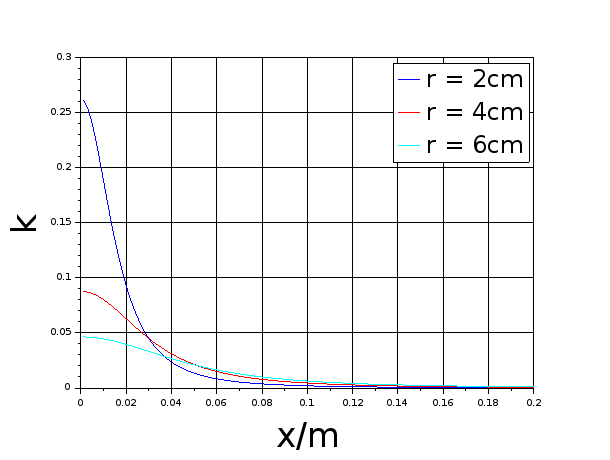
\includegraphics[width=0.9\textwidth]{Graphics/KopplungX.png}
    \caption{Rechnerisch ermittelte Kopplung versch. Spulenradien}{}
  \label{coupling}
\end{figure}

\noindent Deutlich ist in Abbildung \ref{coupling} erkennbar, dass eine kleine Lesegerätantenne bei sehr geringen Abständen im Vergleich zu den größeren Antennen eine wesentlich höhere Kopplung ermöglicht, aber auch mit zunehmender Distanz erheblich schneller abfällt. Ideal ist ein Spulenradius \(r_1\) offensichtlich genau dann, wenn gilt

\begin{equation}
  r_1 \approx x
\end{equation}

\noindent Auch ist eine möglichst große Antenne nicht immer die beste Wahl. Der Vorteil einer größeren Antenne liegt darin, dass die Kopplung mit steigender Distanz weniger stark abfällt. Wird also von einem System erwartet, dass es sowohl bei geringen als auch bei höheren Distanzen zuverlässig arbeitet, ist eine größere Antenne von Vorteil. Zu dem gleichen Ergebnis sind Gerhard Schalk und Renke Bienert in ihrem Buch "RFID MIFARE und kontaktlose Smartcards angewandt" in einem ähnlichen Test gekommen. Schalk und Bienert haben ermittelt welcher Spulenradius für feste Distanzen ideal ist\footnote{Vgl. Schalk, Gerhard und Bienert, Renke: RFID MIFARE und kontaktlose Smartcards angewandt. 1. Auflage: Elektor-Verlag, S. 81}.


}
\endgroup}
%----------------------------------------------------------------------------------------
